\documentclass[10pt]{article}
\usepackage{icmlko}

\icmlmeta{IP 파운데이션 월드모델}{188}{무리별로는 되고 합치면 안 된다}{노트 187의 재현 실험을 위키까지 넓혔다. 무리 하나만 놓으면 트리의 96\%가 재현되는데, 다섯 무리를 합칠 방법을 못 찾았다 --- 새 정식화 하나를 만들어 붙였고 졌다}

\begin{document}

\twocolumn[
\icmlheader

\begin{abstract}
노트 187이 달력에서 ``도메인별 계수 $\times$ 짝 곱''이 트리의 88\%를
재현하는 것을 보이고 위키를 남겼다. 위키 · 검색에 같은 처방을 댔다.
\textbf{된다 --- 96\%다.} 그리고 어느 곱이 일하는지 갈랐다. \textbf{무리
안 곱이 전부다} --- 주효과 $+$0.2748 · \textbf{무리 안 곱만 $+$0.3103} ·
무리 사이 곱만 $+$0.2745(주효과와 같다) · 트리 $+$0.3118. 위키끼리 · 검색끼리
곱하는 것은 값을 하고 위키$\times$검색은 한 톨도 안 낸다. 그래서 처방을
전체 열아홉 축에 댔다. \textbf{무너진다} --- 무리 안 곱만 골라 넣어도 열이
쉰여섯이 되고 판이 $+$0.3908 에서 \textbf{$+$0.3582} 로 \emph{내려간다}.
주효과가 이미 설명한 분산 위에 곱 서른일곱을 얹는 것이라 잡음만 는다.
\textbf{무리별로는 되고 합치면 안 된다.} 그래서 합치는 정식화를 만들었다 ---
\textbf{F19 무리 쌓기}는 1단에서 무리마다 (도메인별 절편 $+$ 무리 안 곱)
능형을 접힘 밖으로 적합하고 2단에서 그 예측 다섯을 다시 섞는다.
\textbf{졌다} --- $+$0.3758 로 F10 도메인별($+$0.3914)보다도 낮고 챔피언
F18($+$0.4490)에는 $-$0.0732($t{=}-6.78$)다. 웹툰 $-$0.153 · 아이돌
$-$0.169 로 무너진다. \textbf{그러니 이 사이클의 결론은 부정형이다} ---
트리가 무리 안에서 하는 일은 알아냈고(도메인별 $\times$ 곱), 무리를 가로질러
하는 일은 못 알아냈다. 남는 가설 하나: \textbf{트리는 무리를 \emph{곱}하지
않고 \emph{조건}한다.} 무리 사이 곱이 0 을 낸 것과 모순이 아니다 --- ``위키
값이 크면 그다음 달력을 본다''는 곱으로 못 쓴다.
\end{abstract}
]

\begin{figure*}[t]
\centering
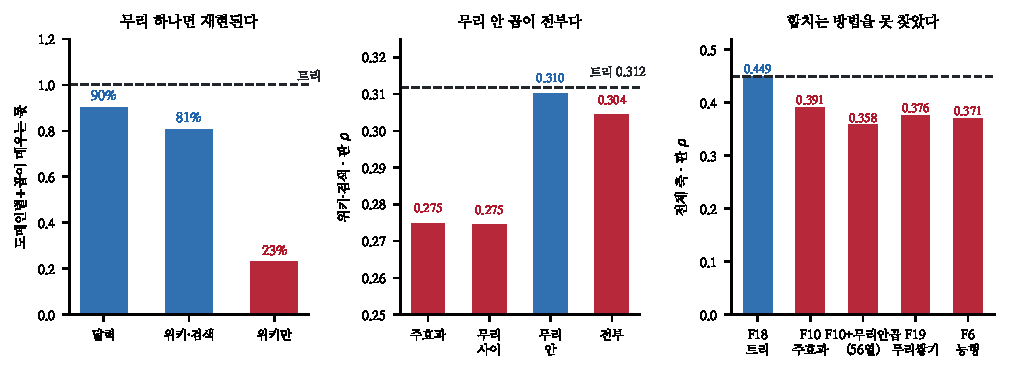
\includegraphics[width=\textwidth]{figs/stack.pdf}
\caption{왼쪽 --- 무리 하나면 재현된다. 가운데 --- 무리 안 곱이 전부다.
오른쪽 --- 합치는 방법을 못 찾았다.}
\end{figure*}

\section{무리 하나면 재현된다}

\begin{table}[t]
\centering\tsize
\caption{무리별. 도메인별 계수 $+$ 무리 안 짝 곱.}
\begin{tabular}{lrrrr}
\toprule
& 풀링 & 도메인별$+$곱 & 트리 & 메움 \\
\midrule
달력 & $-$.024 & $+$.100 & $+$.114 & \textbf{90\%} \\
\textbf{위키·검색} & $+$.274 & $+$.304 & $+$.312 & \textbf{81\%} \\
위키만 & $+$.119 & $+$.131 & $+$.172 & 23\% \\
\bottomrule
\end{tabular}
\end{table}

\claimx{\textbf{위키만 놓으면 23\%밖에 안 메워진다.} 위키 넷에 검색 넷을
같이 놓으면 81\%다 --- 열이 여덟이라 무리 안 곱이 스물여덟에서 여섯으로
줄지 않는다.}{처음엔 ``위키$\times$검색 교차가 일한다''로 읽었다. 갈라
보니 아니다 --- 다음 절.}

\section{무리 안 곱이 전부다}

\begin{table}[t]
\centering\tsize
\caption{위키·검색 여덟 열. 곱을 갈라 넣는다.}
\begin{tabular}{lrrr}
\toprule
& 열 & 도메인별 & 풀링 \\
\midrule
주효과만 & 8 & .2748 & .2735 \\
\textbf{무리 사이 곱만} & 24 & \textbf{.2745} & .2710 \\
\textbf{무리 안 곱만} & 20 & \textbf{.3103} & .2903 \\
곱 전부 & 36 & .3044 & .2808 \\
\midrule
\textbf{트리} & 8 & \textbf{.3118} & \\
\bottomrule
\end{tabular}
\end{table}

\claimx{\textbf{무리 사이 곱은 한 톨도 안 낸다}($+$0.2745 대 주효과
$+$0.2748). \textbf{무리 안 곱만 넣으면 트리의 96\%가 온다}($+$0.3103 대
$+$0.3118).}{위키 넷은 같은 시계열에서 뽑은 수준 · 기울기 · 변동 · 봉우리비다.
그것끼리의 곱은 ``높은데 요동친다'' 같은 모양을 만든다. 위키$\times$검색은
서로 다른 창구의 관심도라 곱해도 뜻이 안 생긴다.}

\claimx{\textbf{곱을 다 넣으면 오히려 준다}($+$0.3044 대 $+$0.3103). 쓸모없는
무리 사이 곱 열여섯이 잡음만 더한다.}{\textbf{어느 곱을 넣느냐가 몇 개를
넣느냐보다 중요하다.}}

\section{합치면 무너진다}

\begin{table}[t]
\centering\tsize
\caption{전체 열아홉 축. 무리 안 곱만 골라 넣어도.}
\begin{tabular}{lrr}
\toprule
& 열 & 판 $\rho$ \\
\midrule
F10 주효과 & 19 & \textbf{.3908} \\
F10 $+$ 무리 안 2차 & 56 & \textbf{.3582} \\
F10 $+$ 무리 안 2·3차 & 94 & .3296 \\
\bottomrule
\end{tabular}
\end{table}

\claimx{\textbf{내려간다.} 무리별로 하면 되던 것이 다 넣으면 안 된다 ---
쉰여섯 열이면 유보가 도메인당 스물다섯에서 칠백인 판에 과하다.}{내 예측이
틀렸다 --- $+$0.42$\sim$$+$0.45 를 적었다. \textbf{걸어 둔 반대 가능성
(``쉰여섯이면 과적합한다'')이 또 맞았다} --- 세 사이클 연속이다(노트 180 ·
181 · 188).}

\section{합치는 정식화를 만들었고 졌다}

\begin{table}[t]
\centering\tsize
\caption{F19 무리 쌓기. 1단 무리별 접힘 밖 $\to$ 2단 혼합.}
\begin{tabular}{lrl}
\toprule
& 판 $\rho$ & \\
\midrule
\textbf{F18 배깅} & \textbf{.4490} & 챔피언 \\
F10 도메인별 & .3914 & \\
\textbf{F19 무리 쌓기} & \textbf{.3758} & $-$.0732 ($t{=}-6.78$) \\
F6 능형 & .3709 & \\
\bottomrule
\end{tabular}
\end{table}

\claimx{\textbf{도전자가 졌다.} F10 주효과보다도 낮다. 웹툰 $-$0.153 ·
아이돌 $-$0.169 로 무너지고 펀딩($+$0.052) · 팝업($+$0.011)에서만
얻는다.}{2단이 무리 예측 다섯을 도메인별 절편과 함께 선형으로 섞는데,
\textbf{그 혼합 자체가 도메인마다 조건부여야 하는지도 모른다} --- 웹툰이
제일 크게 무너지는 것이 그 방향을 가리킨다(노트 182: 웹툰은 자기 과거를
못 쓴다).}

\claimx{\textbf{그래도 포트폴리오에 남긴다.} 노트 125가 세운 규약대로
도전자는 지더라도 등록하고 점수를 남긴다 --- 나중에 자료가 바뀌면 다시
붙는다.}{F19 가 이긴 두 도메인이 유보 팔십과 쉰아홉짜리 작은
도메인이라는 것도 적어 둔다. \textbf{노트 183의 그늘로 보면 F19 는 작은
도메인에 친절하고 큰 도메인에 잔인하다.}}

\section{남는 가설}

\claimx{\textbf{트리는 무리를 곱하지 않고 조건한다.} 무리 사이 곱이 0 을
낸 것과 모순이 아니다 --- ``위키 값이 크면 그다음 달력을 본다''는 곱으로
표현이 안 된다. 곱은 대칭이고 조건은 순서가 있다.}{그러면 재현하려면 곱이
아니라 \emph{쪼갬}이 필요하고, 그건 결국 트리다. \textbf{해석 가능한
모형으로 챔피언을 흉내 내는 길이 여기서 막힐 수도 있다.}}

\begin{table}[t]
\centering\tsize
\caption{남은 것.}
\begin{tabular}{ll}
\toprule
\textbf{조건부} & 무리 사이 쪼갬을 명시로 넣으면 \\
2단 & 혼합 자체를 도메인별 조건부로 \\
열 수 & 무리별로 곱을 고르는 규칙 \\
\bottomrule
\end{tabular}
\end{table}

첫 줄이 곧바로 잴 수 있다. 무리 사이 \emph{쪼갬}은 곱보다 표현하기 쉽다 ---
무리 하나의 예측을 몇 구간으로 자르고 그 구간을 다른 무리의 계수에
곱하면 된다. \textbf{그것이 되면 ``트리는 조건한다''가 맞고, 안 되면 트리의
남은 우위는 깊이 셋 이상의 조합이다} --- 후자면 해석 가능한 재현을 포기하고
노트 185의 결론(공유 축에서는 선형으로 충분하다)으로 만족하는 것이 맞다.

\end{document}
